\section{XML Encryption}
The information here was taken from a couple of different
sources.~\autocite{w3c_xml_encryption} XML encryption is a standard created by
W3C to allow for a standardized way of containing encrypted data in XML\@. In
order for it to work the following components should be present:

\begin{description}
    \item[Application] The application which makes request of an XML Encryption
        implementation via the provision of data and parameters necessary for
        its processing.
    \item[Encryptor] An XML Encryption implementation with the role of encrypting
        data.
    \item[Decryptor] An XML Encryption implementation with the role of decrypting
        data.
\end{description}
\subsection{Usages}
An important feature of XML Encryption is that it can be used directly in XML\@.
Which makes it possible to encrypt just some elements or some content of
elements instead of the full XML file. Encrypting arbitrary data is also
supported however.
\subsection{EncryptedData}
XML Encryption uses the EncryptedData node which contains the encrypted data and
optionally information needed to decrypt it, like the encryption algorithm that
was used.

When encrypting an XML element or element content the EncryptedData element
replaces the element or content (respectively) in the encrypted version of the
XML document.

When encrypting arbitrary data (including entire XML documents), the
EncryptedData element may become the root of a new XML document or become a
child element in an application-chosen XML document.

An XML document may contain zero or more EncryptedData elements. EncryptedData
cannot be the parent or child of another EncryptedData element.
\subsubsection{Syntax}
\begin{minted}{xml}
<EncryptedData Id? Type? MimeType? Encoding?>
  <EncryptionMethod/>?
  <ds:KeyInfo>
    <EncryptedKey>?
    <AgreementMethod>?
    <ds:KeyName>?
    <ds:RetrievalMethod>?
    <ds:*>?
  </ds:KeyInfo>?
  <CipherData>
    <CipherValue>?
    <CipherReference URI?>?
  </CipherData>
  <EncryptionProperties>?
</EncryptedData>
\end{minted}

The CipherData element envelopes or references the raw encrypted data. If
enveloping, the raw encrypted data is the CipherValue element's content; if
referencing, the CipherReference element's URI attribute points to the location
of the raw encrypted data

\subsection{Examples}
The example code here was taken from the W3C spec~\autocite{w3c_xml_encryption}.
When looking at this xml file it is clear that it contains sensitive
information.

\begin{minted}{xml}
  <?xml version='1.0'?>
  <PaymentInfo xmlns='http://example.org/paymentv2'>
    <Name>John Smith</Name>
    <CreditCard Limit='5,000' Currency='USD'>
      <Number>4019 2445 0277 5567</Number>
      <Issuer>Example Bank</Issuer>
      <Expiration>04/02</Expiration>
    </CreditCard>
  </PaymentInfo>
\end{minted}

The first way to remove this is by encrypting an the whole creditcard element.

\begin{minted}{xml}
  <?xml version='1.0'?>
  <PaymentInfo xmlns='http://example.org/paymentv2'>
    <Name>John Smith</Name>
    <EncryptedData Type='http://www.w3.org/2001/04/xmlenc#Element'
     xmlns='http://www.w3.org/2001/04/xmlenc#'>
      <CipherData>
        <CipherValue>A23B45C56</CipherValue>
      </CipherData>
    </EncryptedData>
  </PaymentInfo>
\end{minted}

A second way is to encrypt the content of the CreditCard element.

\begin{minted}{xml}
  <?xml version='1.0'?>
  <PaymentInfo xmlns='http://example.org/paymentv2'>
    <Name>John Smith</Name>
    <CreditCard Limit='5,000' Currency='USD'>
      <EncryptedData xmlns='http://www.w3.org/2001/04/xmlenc#'
       Type='http://www.w3.org/2001/04/xmlenc#Content'>
        <CipherData>
          <CipherValue>A23B45C56</CipherValue>
        </CipherData>
      </EncryptedData>
    </CreditCard>
  </PaymentInfo>
\end{minted}

Finally it is possible to encrypt the full file, not even showing what the file
is about.

\begin{minted}{xml}
  <?xml version='1.0'?>
  <EncryptedData xmlns='http://www.w3.org/2001/04/xmlenc#'
   MimeType='text/xml'>
    <CipherData>
      <CipherValue>A23B45C56</CipherValue>
    </CipherData>
  </EncryptedData>
\end{minted}


\subsection{Encryption Algorithms}
\subsubsection{Symmetric}
\begin{itemize}
    \item Most common type of cryptographic algorithms (also called private key
        cryptography)
    \item Use a single key to encrypt and decrypt a message
    \item With symmetric encryption, algorithms are designed to decrypt the
\end{itemize}
An important thing to note is that It is essential that the key is kept
confidential. In case an attacker secured the key, he/she could decrypt any
messages transfered.
\begin{minted}{xml}
    <EncryptedData xmlns='http://www.w3.org/2001/04/xmlenc#'
        Type='http://www.w3.org/2001/04/xmlenc#Element'/>
  [s2]   <EncryptionMethod
          Algorithm='http://www.w3.org/2001/04/xmlenc#tripledes-cbc'/>
         <ds:KeyInfo xmlns:ds='http://www.w3.org/2000/09/xmldsig#'>
  [s4]     <ds:KeyName>John Smith</ds:KeyName>
         </ds:KeyInfo>
  [s6]   <CipherData><CipherValue>DEADBEEF</CipherValue></CipherData>
       </EncryptedData>
\end{minted}
See Table~\vref{tab:encrypted_data} for an explanation on the different tags.

\begin{table}
    \begin{tabulary}{\textwidth}{cL}
        \toprule
        Label & Explanation \\
        \midrule
        s2 & This (3DES CBC) is a symmetric key cipher. \\

        s4 & The symmetric key has an associated name ``John Smith''. \\

        s6 & CipherData contains a CipherValue, which is a base64 encoded octet
        sequence. Alternately, it could contain a CipherReference, which is a
        URI reference along with transforms necessary to obtain the encrypted
        data as an octet sequence. \\
        \bottomrule
    \end{tabulary}
    \caption{Explanation of the tags inside
    EncryptedData}\label{tab:encrypted_data}
\end{table}

\subsubsection{Asymmetric}
Asymmetric encryption (or public key cryptography) uses two keys instead of one

\begin{enumerate}
    \item The private key typically is used to encrypt the message
    \item The public key is used to decrypt the message
\end{enumerate}
See Figure~\vref{fig:public_key} for a simple explanatory image.

\begin{figure}
    \center{}
    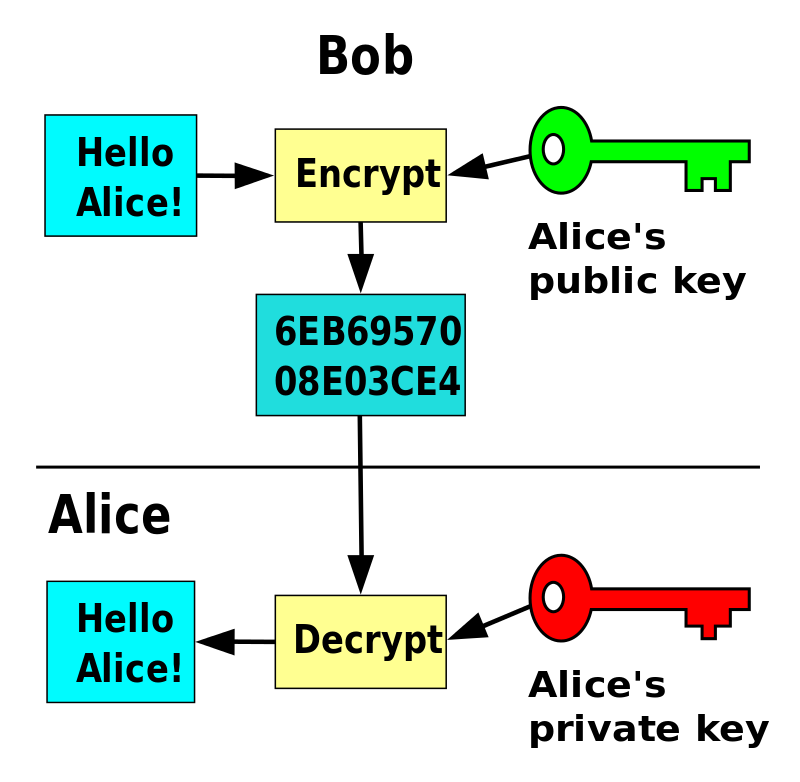
\includegraphics[width=0.5\textwidth]{public_key}
    \caption{Bob encrypts his message with Alice's public
    key\protect\footnotemark}\label{fig:public_key}
\end{figure}
\footnotetext{\url{https://upload.wikimedia.org/wikipedia/commons/thumb/f/f9/Public_key_encryption.svg/800px-Public_key_encryption.svg.png}}
